%\part{Konstruktion}
%\chapter{Programmlogik}
%\section{QueryResolution}

\subsection{QueryBuild}

\begin{figure}[htb]
  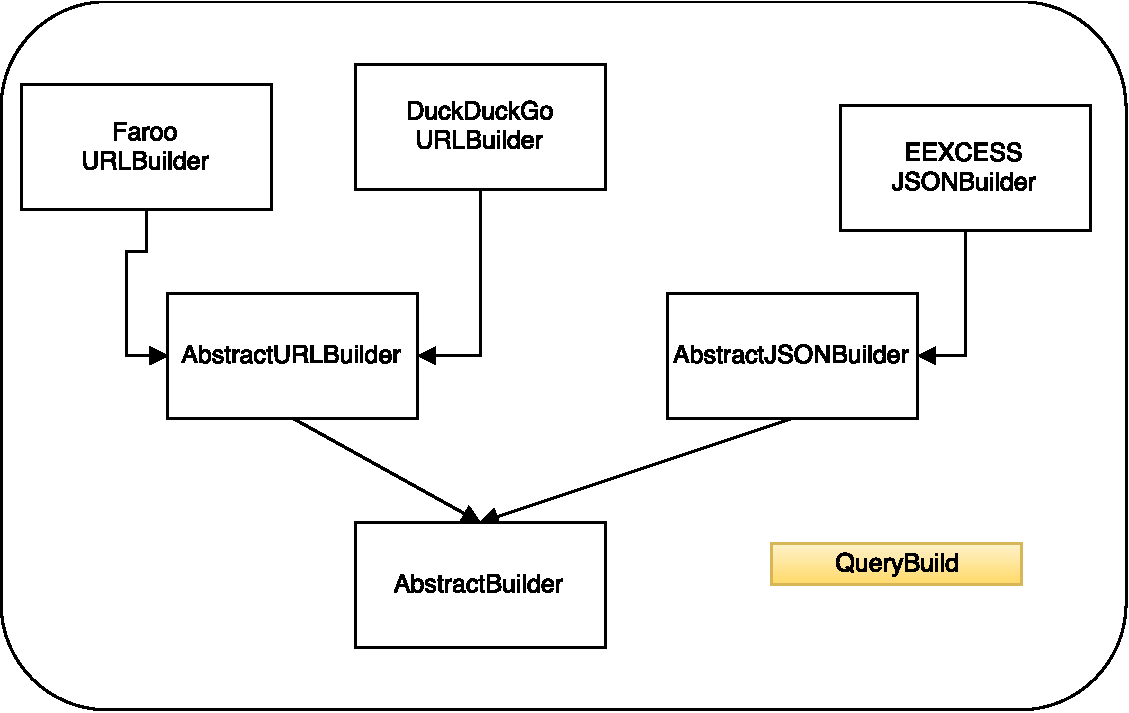
\includegraphics[width=\textwidth]{qr_querybuild}
  \caption{Aufbau des Moduls \lstinline|QueryBuild|}
	\label{fig:Aufbau des Moduls \lstinline|QueryBuild|}
\end{figure}

Das Modul \lstinline|QueryBuild| liefert den größten Teil der Intelligenz im Modul \lstinline|QueryResolution|. Die Aufgaben des Moduls sind es, die \lstinline|ConnectionController| in \lstinline|QuerySend| zu konfigurieren, die Query in das suchmaschinenspezifische Anfrageformat umzuwandeln und dem \lstinline|ConnectionController| den Parser für die Antwort zu geben.

Es gibt für jede Suchmaschine eine Implementation der Spezifikation \lstinline|AbstractBuilder|, welche durch die Spezifikationen \lstinline|URLAbstractBuilder| und \lstinline|JSONAbstractBuilder| erweitert wird.

\subsubsection{AbstractBuilder}
\subsubsection{AbstractJSONBuilder}
\subsubsection{AbstractURLBuilder}
\subsubsection{EexcessJSONBuilder}
\subsubsection{FarooURLBuilder}
\subsubsection{DuckDuckGoURLBuilder}
\subsubsection{EEXCESSOrigin}

%\paragraph{Paragraph}
%\subparagraph{Unterparagraph}
